    Теперь попробем посчитать по определению сингулярные гомологии для какого-нибудь пространства. 
    Оказывается, что по определению сделать это возможно разве что для точки.

    \begin{theorem}[Сингулярные гомологии точки]
        \[ H_{q}^{\mathrm{sing}}(*, \Z) = 0, \ H_{0}^{\mathrm{sing}}(*, \Z) = \Z, \ \widetilde{H}_{0}^{\mathrm{sing}}(*, \Z) = 0. \]
    \end{theorem}
      Итак, как мы помним, $C_{q}(*)$~--- все линейные комбинации отображений $f\colon T^{q} \to *$.
    Так как отображений из $T^n$ в точку всего одно, $\forall n \ C_{n}(X, \Z)  = \Z$, а значит, наш комплекс
    сингулярных цепей $(C_{\bullet}(*, \Z), \partial)$ будет иметь вид:
    \[ \ldots \Z \xrightarrow{\partial} \Z \xrightarrow{\partial} \ldots \xrightarrow{\partial_2} \Z \xrightarrow{\partial_{1}} \Z \xrightarrow{\varepsilon} \Z. \]
    Теперь посчитаем дифференциалы комплекса.

    Возьмем $f \in C_{1}$, это какая-то формальная линейная комбинация отображений из $[a, b] \to \{ * \}$ Тогда $\partial f$~--- это
    $f\vert_{a} - f\vert_{b} = 0$. Впрочем, и сразу ясно, что в случае любого $n$, так как наше отображение действует в точку (оно постоянно),
    сужения на все грани будут совпадать и результат в сумме будет зависеть лишь от четности $n$, то есть дифференциалы комплекса будут иметь вид:
    \[ \ldots \Z \xrightarrow{\cdot 0} \Z \xrightarrow{\cdot 1} \ldots \xrightarrow{\cdot 1 = \mathrm{id}} \Z \xrightarrow{0} \Z \xrightarrow{\varepsilon} \Z \]
    Иными словами, $\partial_n = 0$, если $n$~--- нечетное и тождественно иначе. Теперь, как нетрудно заметить,
    \[ \forall q > 0 \quad \Ker{\partial_{q}} = \Im{\partial_{q + 1}} \Rightarrow H_{q}^{\mathrm{sing}}(*, \Z) = 0, \ H_{0}^{\mathrm{sing}}(*, \Z) = \Z, \ \widetilde{H}_{0}^{\mathrm{sing}}(*, \Z) = 0. \]


    Трудности, возникшие при подсчетах, намекают на то, что для отрезка, например, это будет сделать еще гораздо труднее.
    С другой стороны, если вдруг окажется, что гомологии гомотопически инвариантны, то мы будем знать, какие гомологии у всех
    стягиваемых пространств (так как для точки мы посчитали).

    В дальнейшем, будем использовать для сингулярных гомологий обозначение $H_{k}$.

    \subsection{Немного гомологической алгеры}

    Рассмотрим категорию цепных комплексов $\fC\fh$ (в нашем случае абелевых групп, но в принципе, всё что тут будет сказано справделиво и в случае $R-\fM\fo\fd$).
    Морфизмом цепных комплексов $(C_{\bullet}, \partial)$ и $(D_{\bullet}, \delta)$ называется набор отображений $f = \{ f_i \}$, где $f_i \in \Hom(C_i, D_i)$ такой, что
    диаграмма
    \begin{center}
        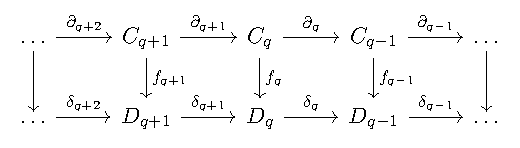
\includegraphics{lectures/0/pictures/cd_1}
    \end{center}
    коммутативна, то есть $\forall i \ f_{i} \circ \partial_{i + 1} = \delta_{i + 1} \circ f_{i + 1}$.

    \begin{lemma}
        Сопоставление цепному комплексу его $k$-й группы гомологий функториально, то есть отображение
        \[ (C_{\bullet}, \partial) \mapsto H_{k}(C_{\bullet}, \delta) \]
        задаёт ковариантный функтор $\fC\fh \to \fA\fb$.
    \end{lemma}
    \begin{proof}
        Всё, кроме того, что композиция переходит в композицию~--- совсем очевидно.
        Нам надо проверить, что отображение $(C_{\bullet}, \partial) \xrightarrow{f} (D_{\bullet}, \delta)$ индуцирует отображение
        $H_{k}(C_{\bullet}) \to H_{k}(D_{\bullet})$, и кроме того,
        \[ (C_{\bullet}, \partial) \xrightarrow{f} (D_{\bullet}, \delta) \xrightarrow{g} (E_{\bullet}, d) \Rightarrow H_{k}(f \circ g) = H_{k}(f) \circ H_{k}(g).\]

        Заметим, что так как $f \in \Hom(C_{\bullet}, D_{\bullet})$, $f_{q}(\Ker{\partial_{q}}) \subset \Ker{\delta_{q}}$.
        Действительно, если $\partial_{q}(x) = 0$, то $0 = f_{q - 1}(\partial_{q}(x)) = \delta_{q}(f_{q}(x)) \Rightarrow f_{q}(x) \in \Ker{\delta_{q}}$.
        Аналогично $f_{q - 1}(\Im{\partial_{q}}) \subset \Im{\delta_{q}}$. Действительно, если $x = \partial_{q}(y)$, то
        \[ f_{q - 1}(x) = f_{q - 1} \circ \delta_{q}(x) = \delta_{q}(f_{q}(y)) \in \Im{\delta_{q}}. \]
        Тогда нужная нам стрелка получается просто из универсального свойства факторгруппы:
        \begin{center}
            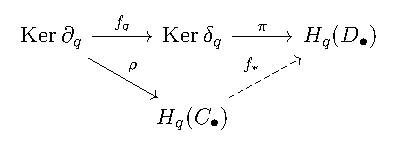
\includegraphics{lectures/0/pictures/cd_2}
        \end{center}
        Действительно, чтоб она существовала, нам нужно, чтоб $\Im{\partial_{q + 1}} \subset \Ker(\pi \circ f_{q})$. Возьмем $x \in \Im{\partial_{q + 1}}$, тогда
        $f_{q}(x) \in \Im_{\delta_{q + 1}} \Rightarrow f_{q}(x) \in \Ker{\pi}$, то есть $x \in \Ker{(\pi \circ f_{q})}$.

        Проверка того, что композиция переходит в композицию тривиальна.
    \end{proof}
    
    \begin{remark}
       Пусть $X, Y \in \fT\fo\fp$, $f\colon X \to Y$~--- непрерывное отображение. Тогда оно индуцирует морфизм
       цепных комплексов $f\colon C_{\bullet}(X) \to C_{\bullet}(Y)$. Действительно, пусть $g \in C_{k}(X)$, тогда $g$~--- это
       непрерывное отображение $T_{k} \to X$ и тогда $f \circ g$~--- непрерывное отображение $T_{k} \to Y$, то есть элемент $C_{k}(Y)$.
       Остается проверить, что полученное отоюражение будет коммутировать с дифференциалом.
       \[ \partial g = \sum_{i = 0}^{k} (-1)^{i} \Gamma_{i}g. \]
       Тогда остается заметить, что взятие грани коммутирует с применением отображения:
       \[ f(\partial{g}) = \sum_{i = 0}^{k} (-1)^{i} \Gamma_{i}f(g) = \partial(f g).   \]

        Значит, если у нас есть непрерывное отображение $f\colon X \to Y$, то есть и индуцированный морфизм гомологий $f_{*}\colon H_{\bullet}(X) \to H_{\bullet}(Y)$.
    \end{remark}   
    
    \begin{statement}
        Если $f\colon X \to Y$~--- гомеоморфизм, то $f_{*}\colon H_{k}(X) \to H_{k}(Y)$~--- изоморфизм (для всех $k$). 
    \end{statement}
    \begin{proof}
        Действительно, если $f$~--- гомеоморфизм, то все индуцированные отображения между цепями~--- изоморфизмы, а значит и все индуцированные отображения в гомологиях
        будут изоморфизмами.
    \end{proof}
    \begin{remark}
       Это утверждение говорит нам о том, что сингулярные гомологии определены для топологических пространств без всякой дополнительной структуры.
    \end{remark}

    \begin{definition}
        Пусть $X$~--- топологическое пространство. Тогда, если группа  $H_{k}(X)$ конечнопорождена, то
        \[ H_{k}(X) \cong \Z^{n} \oplus \mathrm{Tor}(H^{k}(X)). \]
        Тогда число $n$ (то есть, ранг свободной части) называют $k$-м числом Бетти $b_n$. Иными словами, $b_{k}(X) = \rank(H_{k}(X))$.
    \end{definition}

    
    \subsection{Гомотопическая инвариантность гомологий}

    \begin{definition}
        Пусть $(C_{\bullet}, \partial), (D_{\bullet}, \delta) \in \fC\fh$~--- два цепных комплекса. Их морфизмы $f, g \in \Hom_{\fC\fh}((C_{\bullet}, \partial), (D_{\bullet}, \delta))$
        называются \emph{гомотопными} ($f \sim g$), если сущесвует диагональный морфизм $h\colon C_{\bullet} \to D_{\bullet + 1}$ такой, что
        \[ h_{q - 1}\partial_{q} + \delta_{q + 1} h_{q} = f_{q} - g_{q}.  \]
        \begin{center}
            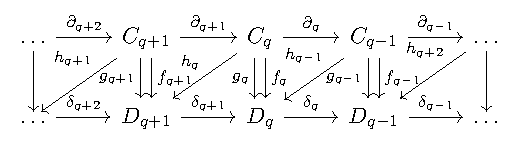
\includegraphics{lectures/0/pictures/cd_3}
        \end{center}
        Кратко это обычно записывают, как $h \partial + \delta h = f - g$.

        Если в категории цепных комплексов $\fC\fh(\fA\fb)$ отождествить гомотопные морфизмы, получится \emph{гомотопическая категория комплексов}, которую обычно обозначают
        $\fK(\fA\fB)$ (или просто $\fK$).
    \end{definition}

    \begin{theorem}\label{HomotopyMorphism}
        Если морфизмы цепных комплексов гомотопны, то есть $f \sim g$, то индуцированные гомоморфизмы когомологий $f_{*} = g_{*}$. Тем самым, функторы гомологий $H_{k}$ пропускаются через гомотопическую категорию.
    \end{theorem}

    \begin{proof}
        Если $x \in \Ker{\partial_{q}}$, то
        \[ f_{q}(x) - g_{q}(x) = \delta_{q + 1} h_{q}(x) + \underbrace{h_{q - 1} \partial_{q}(x)}_{= 0} \in \Im{\delta_{q + 1}},  \]
        а значит в $H_{q}(X)$ эти элементы равны.
    \end{proof}
    \begin{remark}
       Гомотопность морфизмов $f$ и $g$ можно определять, как $\delta h \pm h \partial = f - g$, так как при переходе к гомологиям
       второе слагаемое всё равно обнуляется.
    \end{remark}
    
    \begin{theorem}\label{HomotopyImpliesHomotopy}
        Пусть $f, g\colon X \to Y$, $f \sim g$. Тогда $f_{*} = g_{*}$.
    \end{theorem}
    \begin{proof}
        У нас есть цепные комплексы сингулярных цепей $(C_{\bullet}(X), \partial)$ и $(C_{\bullet}(Y), \partial)$.
        Так как $f \sim g$, существует непрерывное отображение $H\colon X \times I \to Y$, а тогда
        $\forall p\colon T_{q} \to X$ определено непрерывное отобрежение $H(p(\_),\_)\colon T_{q} \times I \to Y$, причем $H(p, 0) = f(p)$
        и $H(p, 1) = g(p)$. Положим
        \[ h(p) = \text{сумма симплексов в разбиении призмы } T_{q} \times I \in C_{q + 1}(Y). \]
        Взглянув на картинку теперь нетрудно заметить, что
        \[ f(p) - h(p) = \text{граница всей призмы} - \text{боковые стенки} = \partial h(p) - h \partial(p) \]
        Таким образом, мы получили, что индуцированные морфизмы цепных комплексов гомотопны, а значит, по теореме~\ref{HomotopyMorphism}, индуцированные
        гомоморфизмы в гомологиях совпадают.
    \end{proof}

    \noindent\bf{Упражнение.}
        Разбить $T_{q} \times I$ на $q + 1$-мерные симплексы формально. А именно, пусть $T_{q} \times \{ 0 \} = a_0 \ldots a_{q}$.
        Пусть вершины $T_{q} \times \{ 1 \}$~--- это $a_0', \ldots, a_q'$. Тогда предлагается брать вершины $a_{0}\ldots a_k a_k' \ldots a_{q}'$.

    \begin{corollary}\label{HomologiesContractible}
        Пусть $X$~--- стягиваемое. Тогда $\widetilde{H}_{\bullet}(X, \Z) = 0$, или, иными словами,
        $\forall k > 0 \ H_{k}(X, \Z) = 0, \ H_{0}(X, \Z) = \Z$.
    \end{corollary}
    
    \noindent\bf{Упражнение.}
        Придумайте пример нестягиваемого $X$ с нулевыми приведёнными гомологиями. 
    
    \begin{lemma}
       Если $X$~--- линейно связно, то $H_{0}(X) = \Z$.
    \end{lemma}
    \begin{proof}
        Выберем в нашем пространстве некоторую фиксированную точку $a$, тогда
        \[ \lr*{\sum k_i f_i} = \lr*{\sum k_i}a \pmod{\Im{\partial_{1}}}, \text{ (то есть, в } H_{0}(X)) \]
        так как все $f_i$ можно соединить путями (а это отображения $T^{1} = [0, 1] \to X$) с $a$ и значит $\Im{\partial_{1}}$ будет содержать
        все разности $f_i - a$. Значит, $H_{0}(X) \cong \Z$.
    \end{proof}

    \begin{corollary}
        Пусть у топологического пространства $X$ $n$ компонент линейной связности. Тогда
        \[ H_{0}(X) \cong \Z^{n}. \]
    \end{corollary}

    \noindent\bf{Упражнение.}
    Дркажите, что непрерывное отображение между линейно связными пространствами индуцирует изоморфизм нулевых гомологий.


    






    

    

    

